\section{Experimental Results}\label{sec:numerical_examples}
\label{Results1}
In this section we evaluate the performance of the proposed algorithm using a two dimensional model of a quadrotor platform, where the task is to follow predefined trajectories. After defining the numerical model, we first look at the performance of the proposed algorithm when there is a gravity mismatch. In the next step, we investigate knowledge transfer between two different trajectories. Note that for hyperparameter estimation, we use five different wave trajectories and the corresponding feed-forward control signals as examples. These examples are then discarded to avoid overfitting.~\footnote{Source code for generating the experimental results can be downloaded from \href{https://icml_tgp@bitbucket.org/icml_tgp/icml_tgp.git}{bitbucket/icml\_tgp}.}

\subsection{Numerical Model}
As an example consider the two-dimensional model of a quadrotor given by \citet{Schoellig12}:	
\begin{equation}
\begin{aligned}
\ddot{y} &= -f_{\mathrm{coll}} \sin\phi  \\
\ddot{z} &=  f_{\mathrm{coll}}\cos\phi - g  \\
\dot{\phi} &= \omega_{x} 
\end{aligned}
\label{quadrocopterDynamics}
\end{equation}
where state $\state = (y,\dot{y},z,\dot{z},\phi)$. The states $y, z$ are trajectories to be tracked, corresponding to the horizontal and vertical axes and the control input $\sysInput = (f_{\mathrm{coll}}, \omega_x)$, where $f_{\mathrm{coll}} = \sum_{i=1}^{4}f_{i}$ is the collective thrust and $\omega_x$ is rate of change of the angle of attack w.r.t. the x-axis.
Input constraints are given by: 
% expand on this
% Note that derivative constraints \eqref{thrust_rate_constraints} and \eqref{angular_acc_constraints} can hinder learning, unless they are sufficiently relaxed. %Too much details.
\begin{align*}
f_{min} \leq f_i &\leq f_{max}, \\
|\dot{f}_i| \leq &\dot{f}_{max}, \\
|\dot{\phi}| \leq &\dot{\phi}_{max}, \\
|\ddot{\phi}| \leq &\ddot{\phi}_{max}
\end{align*}
The values used throughout the numerical examples are given in the Appendix in Table \ref{table_parameters}. Unmodeled dynamics in quadrotors could be due to parameter mismatch (e.g. gravity difference) or a more general repeating disturbance (e.g. a fan). See Appendix for two examples.

\subsection{Learning under Model Mismatch}
%Measurement noise for the states are assumed to be white Gaussian noise, i.e. $\state_{obs} = \state + \epsilon$, $\epsilon \sim \mathcal{N}(0,\sigma_{n}^{2})$. The variance $\sigma_{n}^{2}$ was set to 0.15 during the simulations.

%\begin{figure}
%\center	
%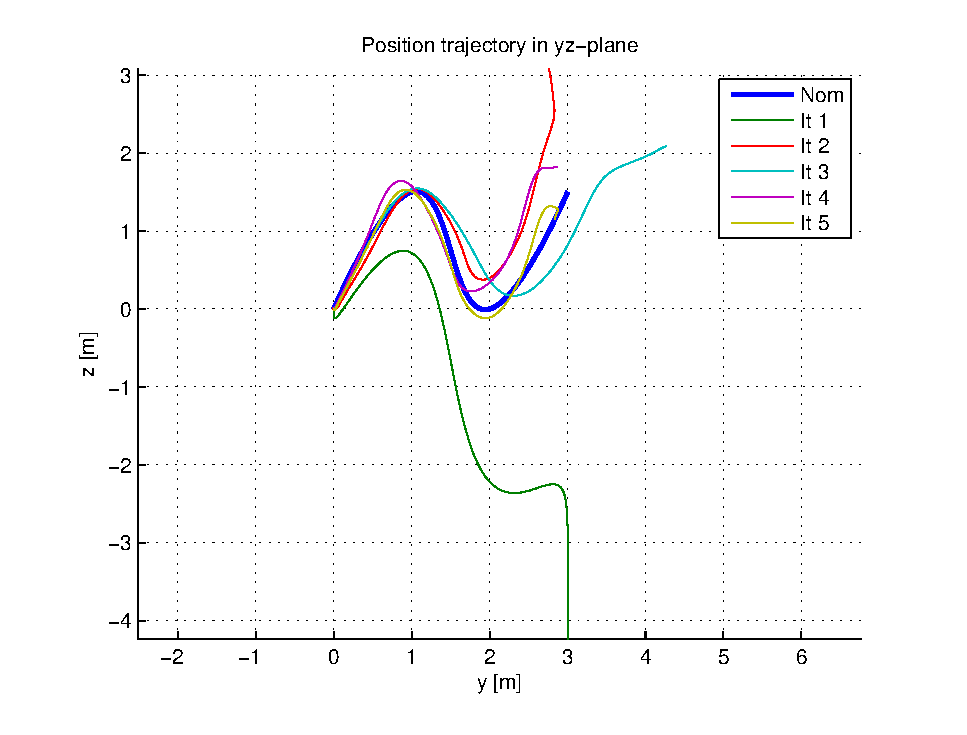
\includegraphics[scale=0.50]{ILCgravity_yz.eps}	
%\caption{Tracking results for ILC under gravity mismatch}
%\label{fig:ilc_x1}
%\end{figure}
%
%\begin{figure}
%\center
%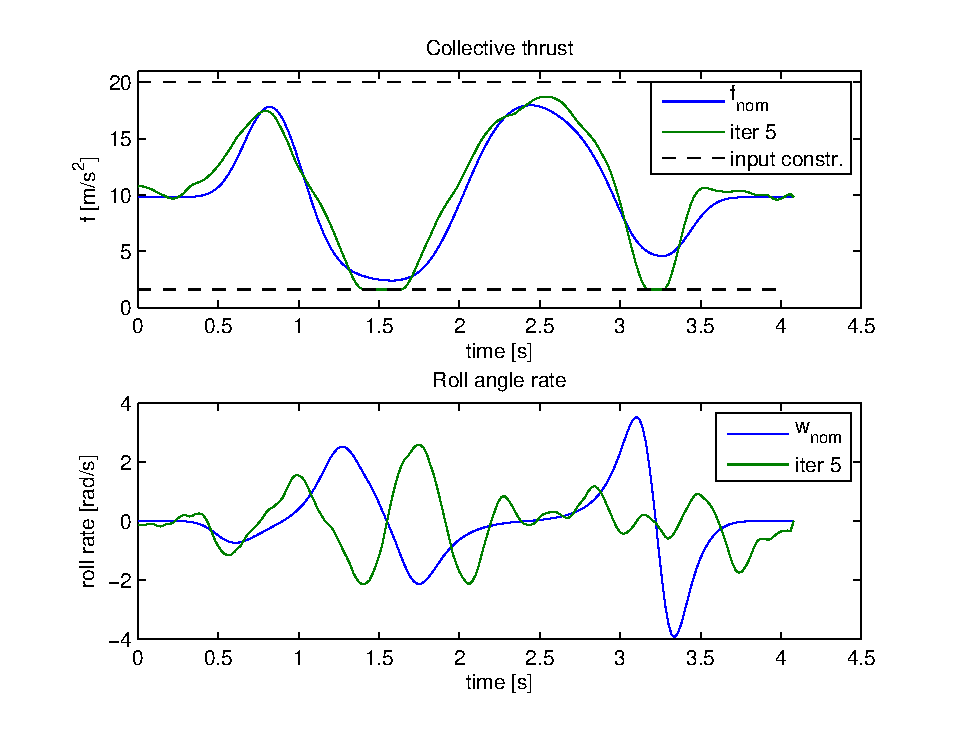
\includegraphics[scale=0.50]{ILCgravity_us.eps}	
%\caption{Control inputs over ILC iterations}
%\label{fig:ilc_u1}
%\end{figure}

%Figure \ref{fig:ilc_u1} shows the change in the control inputs needed to accommodate the gravity mismatch. Only the final input is shown, for better visibility.

Here we show the $\alg$ learning results for the quadrocopter operating under a gravity mismatch. The gravity is taken to be $g_{\mathrm{uranus}} = 10.5$, but the nominal dynamics is assuming earth gravity, $g_{\mathrm{earth}} = 9.81$. We model the cost function \eqref{QuadTheta0} as having bounded RKHS-norm, $\|\cost(\sysInput;\context)\|_{k}^{2} < B$ under the following covariance function:
\begin{align*}
k(\ctxaction, \ctxaction') &= k_u(\sysInput, \sysInput')k_{c}(\context, \context') + \sigma_{n}^{2}\delta_{aa'} \\ 
k_u(\sysInput, \sysInput') &= \sysInput^{\mathrm{T}}\Lambda_{u}^{-2}\sysInput' \\
k_{c}(\context, \context') &= \sigma_{s}^{2}\exp(-\frac{1}{2}(\context-\context')^{\mathrm{T}}\Lambda_{c}^{-2}(\context-\context'))
\end{align*}
where $\ctxaction = (\sysInput;\context)$. Diagonal matrices $\Lambda_{u}$ and $\Lambda_{c_{i}}$ transform anisotropic coordinates into isotropic coordinates or they can be motivated from Automatic Relevance Determination (ARD) point of view where $\Lambda_{u}^{2}$ and $\Lambda_{c}^{2}$ encode the relevance of inputs and contexts, respectively \cite{Rasmussen06}. The bound on the noise, $\sigma_{b}$ was set to 0.15 during the simulations.
%This general structure can be kept for all cases, where model mismatch is expected only in the drift term of the dynamics \eqref{eq:readDynamics}.

In Figure \ref{fig:comparison} we compare the performance of $\alg$ with ILC and (nonlinear) MPC with horizon $M = 5$. Weighted Sum of Squared Errors (SSE) in \eqref{costDiscrete} are plotted to show learning during the first 6 episodes. A weighted squared Euclidean distance is used as the cost function where the diagonal matrix with entries $(1,1,1,1,0.01)$ is taken as the weighting matrix $Q$. The best results for the three algorithms during the episodes are shown in Table \ref{SSE_errors}. Figure \ref{fig:comparison} clearly shows that the method can outperform more conventional methods like MPC when disturbances in the form of unknown dynamics are present, and can compare favorably with feedforward learning controllers like ILC. The yz-trajectories followed during these episodes are plotted in Figure \ref{fig:trajectories}.

\begin{figure}
\center
%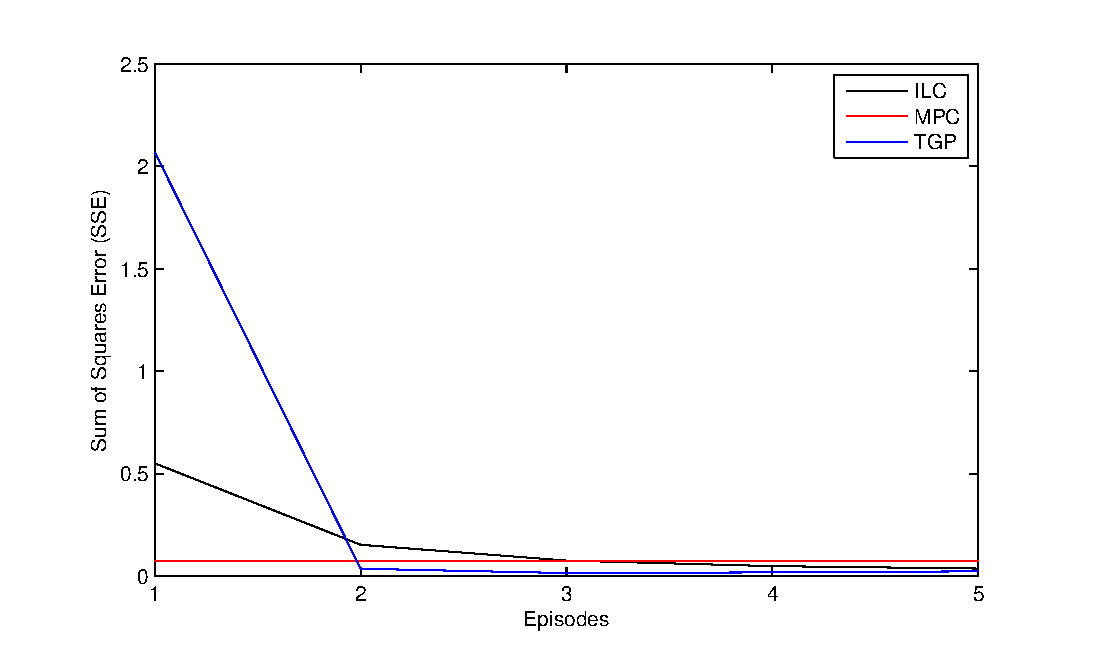
\includegraphics[scale=0.50]{comparison.eps}			
\input{figs/comparision.tikz}
\caption{Comparison of $\alg$, ILC and MPC.}
\label{fig:comparison}
\end{figure}


\begin{figure}
\center	
\input{figs/trajectories.tikz}
\caption{Trajectories $\{(y_t,z_t)\}$ followed by a quadrotor under $\alg$, ILC and MPC: the dashed lines represent the trajectory that needs to be tracked. Solid lines represent the trajectories of the quadrotor tracked by the algorithms. Darker shades of gray represent increasing episodes.}
\label{fig:trajectories}
\end{figure}

\begin{table}[h!t]
% increase table row spacing, adjust to taste
\renewcommand{\arraystretch}{1.3}
\caption{SSE errors}
\label{SSE_errors}
\centering
\begin{tabular}{cc}
\textbf{Method / Episode No.} & SSE \\
\hline
MPC, horizon = 5 & 0.0617 \\
ILC, episode 6 & 0.0306 \\
TGP, episode 6 & 0.0271 \\
\end{tabular}
\end{table}

\subsection{Transfer Learning}

Here we show the transfer learning performance of $\alg$. We implement the scenario considered in section \ref{t-learning} three times using three random wave trajectories: we first run $\alg$ on an initial fixed wave trajectory $\Traj_{0}$ and then switch to a different trajectory $\Traj_{i}$, $i\in{1,2,3}$. Figure \ref{fig:tlearning} shows the tracking error of $\Traj_{i}$ under the transfer learning setting. We compare with TGP running with no prior knowledge and with ILC.

\begin{figure}
\center
%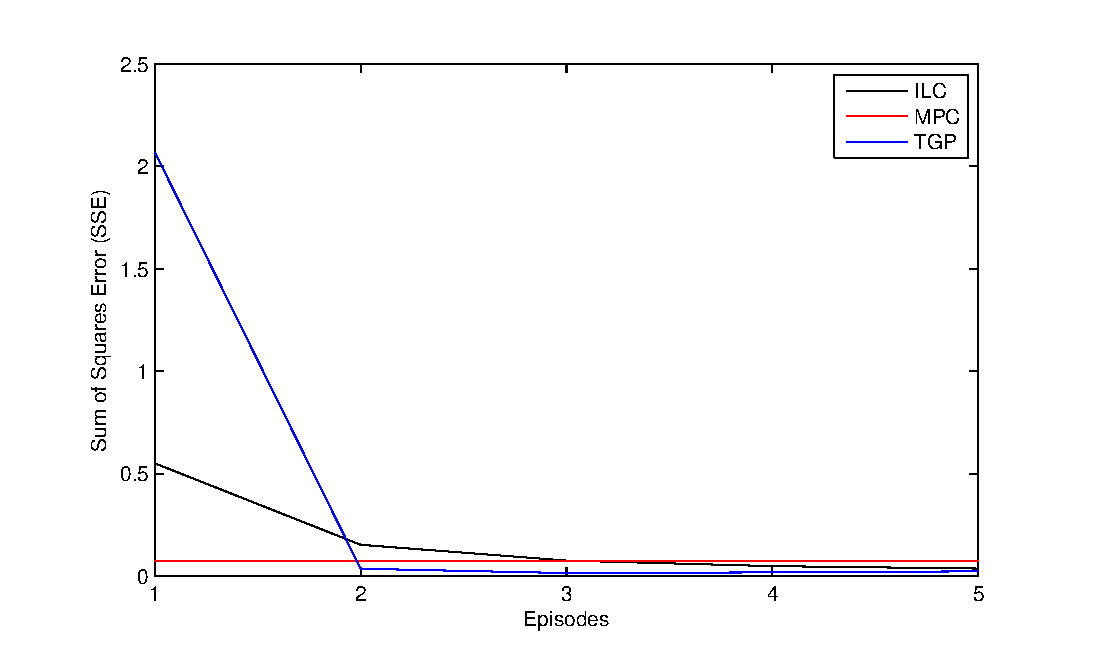
\includegraphics[scale=0.50]{comparison.eps}			
% This file was created by matlab2tikz v0.4.4 running on MATLAB 8.0.
% Copyright (c) 2008--2013, Nico Schlmer <nico.schloemer@gmail.com>
% All rights reserved.
% 
% The latest updates can be retrieved from
%   http://www.mathworks.com/matlabcentral/fileexchange/22022-matlab2tikz
% where you can also make suggestions and rate matlab2tikz.
% 
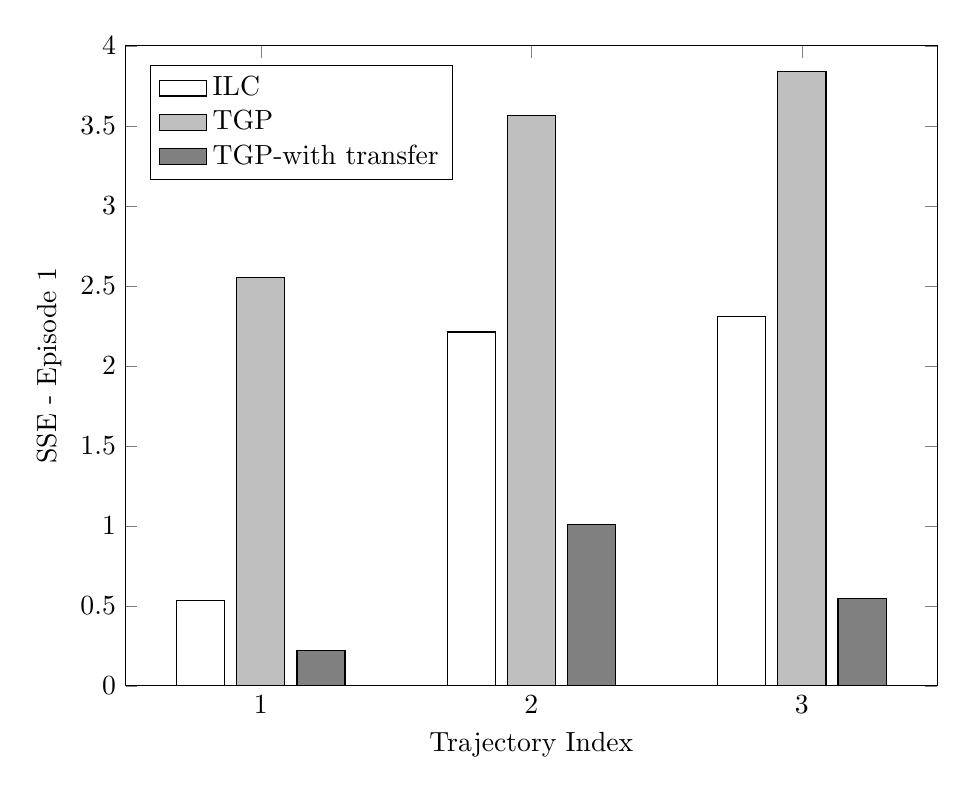
\begin{tikzpicture}

\begin{axis}[%
width=0.85\columnwidth,
height=0.670403225806452\columnwidth,
area legend,
scale only axis,
xmin=0.5,
xmax=3.5,
xtick={1, 2, 3},
xlabel={Trajectory Index},
ymin=0,
ymax=4,
ylabel={SSE - Episode 1},
legend style={at={(0.03,0.97)},anchor=north west,draw=black,fill=white,legend cell align=left}
]
\addplot[ybar,bar width=0.0503703703703704\columnwidth,bar shift=-0.062962962962963\columnwidth,draw=black,fill=white] plot coordinates{(1,0.534257)
(2,2.211294)
(3,2.305692)};

\addlegendentry{ILC};

\addplot [
color=black,
solid,
forget plot
]
table[row sep=crcr]{
0.5 0\\
3.5 0\\
};
\addplot[ybar,bar width=0.0503703703703704\columnwidth,draw=black,fill=lightgray] plot coordinates{(1,2.552392)
(2,3.56266)
(3,3.837903)};

\addlegendentry{TGP};

\addplot[ybar,bar width=0.0503703703703704\columnwidth,bar shift=0.0629629629629629\columnwidth,draw=black,fill=gray] plot coordinates{(1,0.222369)
(2,1.007975)
(3,0.543684)};

\addlegendentry{TGP-with transfer};

\end{axis}
\end{tikzpicture}%
\caption{Comparison of ILC, $\alg$ with and without transfer (from scratch). In the case of \emph{$\alg$ with transfer} the algorithm was first run on a different trajectory.}
\label{fig:tlearning}
\end{figure}


% % % % % % put more plots here % % % % % %